\subsubsection{\stid{4.15} UnifyCR -- A file system for burst buffers} 

\paragraph{Overview} 

The view of storage systems for HPC is changing rapidly. Traditional, 
single-target parallel file systems have reached their cost-effective 
scaling limit. As a result, hierarchical storage systems are being designed 
and installed for our nation's next-generation leadership class systems. 
Current designs employ “burst buffers” as a fast cache between compute 
nodes and the parallel file system for data needed by running jobs and 
workflows. Burst buffers are implemented as compute-node local storage 
(e.g., SSD) or as shared intermediate storage (e.g., SSD on shared burst 
buffer nodes).

Because burst buffers present an additional complexity to effectively
using supercomputers, we are developing UnifyFS, a user-level file system, 
highly-specialized for shared file access on HPC systems with distributed 
burst buffers.  UnifyFS will address a major usability 
factor of current and future systems, because it will enable 
applications to gain the performance advantages from distributed burst buffers 
while providing ease of use similar to that of a parallel file system.


\paragraph{Key  Challenges}

The hierarchical storage for future HPC systems will include compute-node
local SSDs as burst buffers. This distributed burst buffer design promises
fast, scalable I/O performance because burst buffer bandwidth and capacity
will automatically scale with the compute resources used by jobs and
workflows. However, a major concern for this distributed design is how to
present the disjoint storage devices as a single storage location to
applications that use shared files. The primary issue is that when concurrent
processes on different compute nodes perform I/O operations, e.g., writes,
to a shared file, the data for the file are scattered across the separate
compute-node local burst buffers instead of being stored in a single
location. Consequently, if a process wants to access bytes from the
shared file that exist in the burst buffer of a different compute node,
that process needs to somehow track or look up the information for locating
and retrieving those bytes. Additionally, there is no common interface across
vendors for accessing remote burst buffers, so code for cross-node file
sharing will not be easily portable across multiple DOE systems with
different burst buffer architectures, further increasing programming
complexity to support shared files.

For the reasons outlined above, it is clear that without software support 
for distributed burst buffers, applications
will have major difficulties utilizing these resources. 

\begin{figure}[htb]
        \centering
        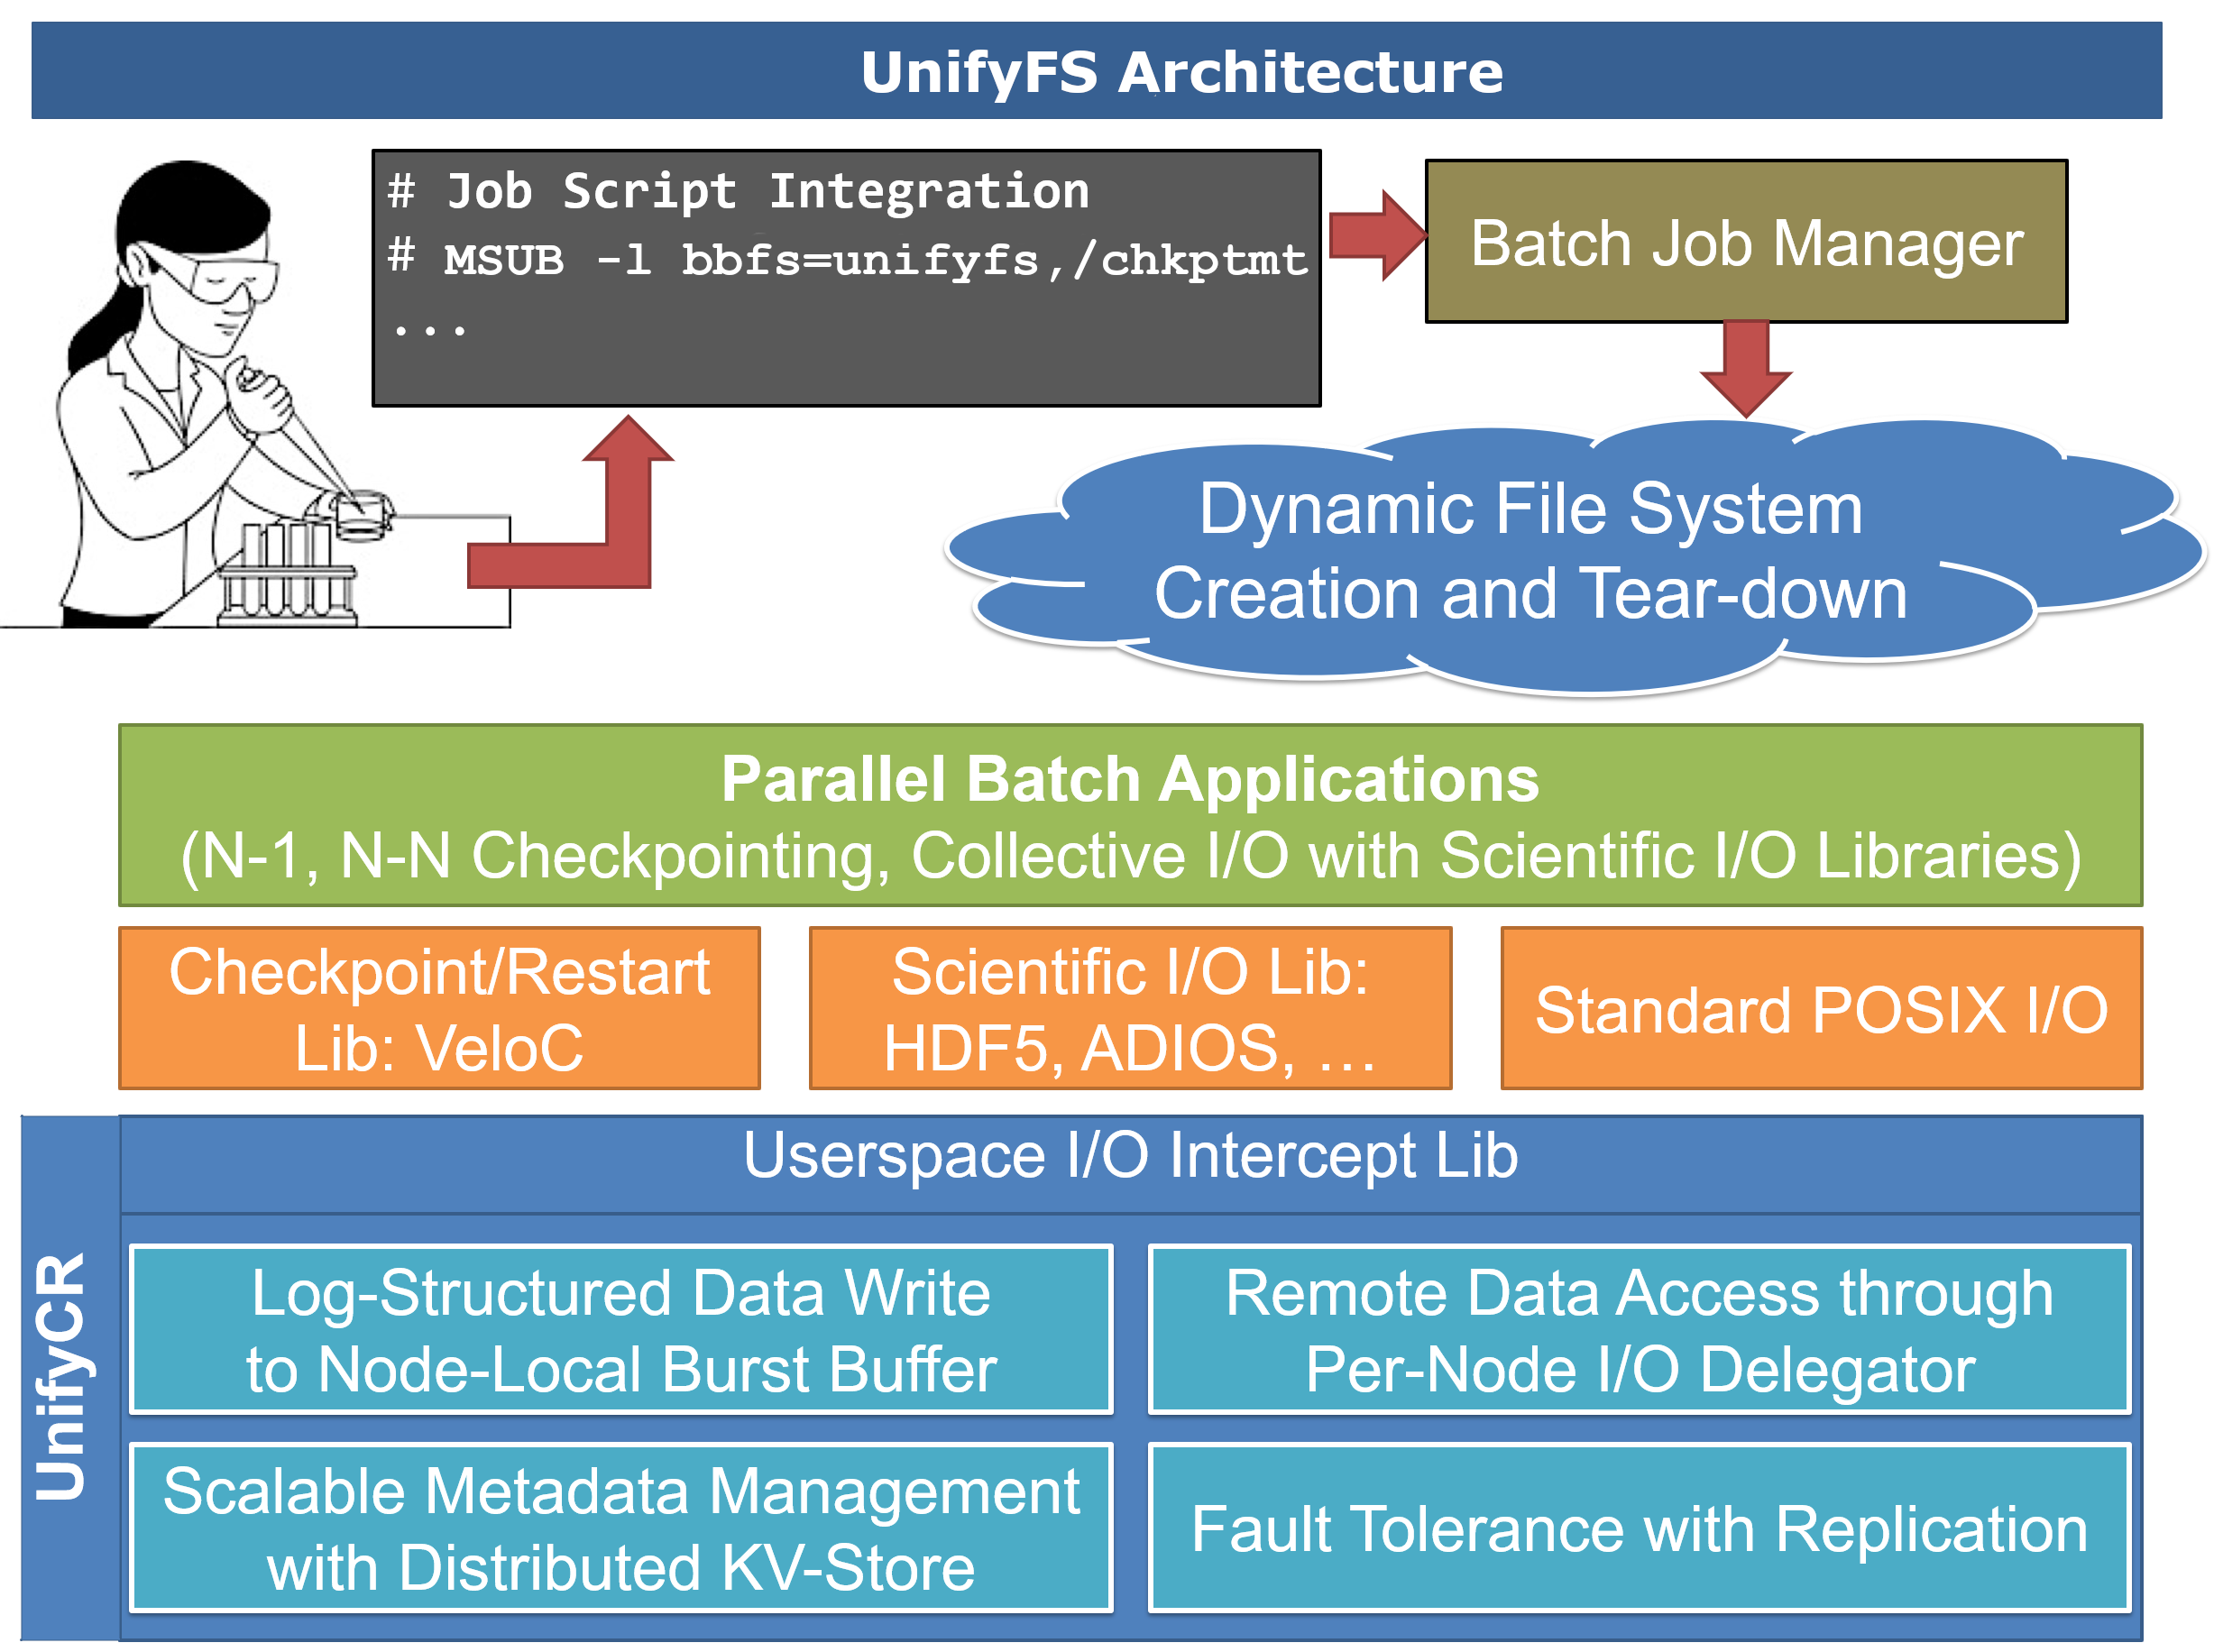
\includegraphics[width=3.5in]{projects/2.3.4-DataViz/2.3.4.15-HDF5-UnifyCR/UnifyFS-overview}
        \caption{\label{fig:UnifyFS-overview} \textbf{UnifyFS Overview.} Users will be able to give commands in their batch scripts to launch UnifyFS within
their allocation. UnifyFS will work with POSIX I/O, common I/O libraries, and
VeloC. Once file operations are transparently intercepted by UnifyFS, they
will be handled with specialized optimizations to ensure high performance.}
\end{figure}

\paragraph{Solution Strategy}

To address this concern, we are developing UnifyFS, a user-level file system,
highly-specialized for shared file access on HPC systems with distributed
burst buffers. In Figure \ref{fig:UnifyFS-overview}, we show a high
level schematic of how UnifyFS works. Users load UnifyFS into
their jobs from their batch scripts. Once UnifyFS is instantiated, user
applications can read and write shared files to the mount point just like
they would the parallel file system. File operations to the UnifyFS
mount point will be intercepted and handled with specialized optimizations
that will deliver high I/O performance. 

Because bulk-synchronous I/O dominates the 
I/O traffic most HPC systems, we target our approach at
those workloads. Examples of bulk-synchronous I/O include checkpoint/restart
and periodic output dumps by appliations. Thus, UnifyFS  addresses a major usability
factor of current and future systems. We designed UnifyFS such
that it transparently intercepts I/O calls, so it will integrate
cleanly with other software including I/O and checkpoint/restart libraries.
Additionally, because UnifyFS is tailored for HPC systems and workloads,
it can deliver high performance.



\paragraph{Recent Progress}

In the third year of this project, the team worked to implement the
design plan that was established in the first
year of the project (See Figure \ref{fig:milestone2}). In particular
we completed the replacement of MPI communication with DataLib software; we developed
support for moving data into and out of UnifyFS by I/O libraries and VeloC;
we implemented and tested support for VeloC; we updated and improved our integration
with resource managers; we furthered our efforts to evaluate and implement support for I/O 
libraries. Additionally, we detected and fixed numerous bugs, improved documentation, and
implemented a metadata abstraction layer, and released UnifyFS 0.9.
\begin{figure}[htb]
        \centering
        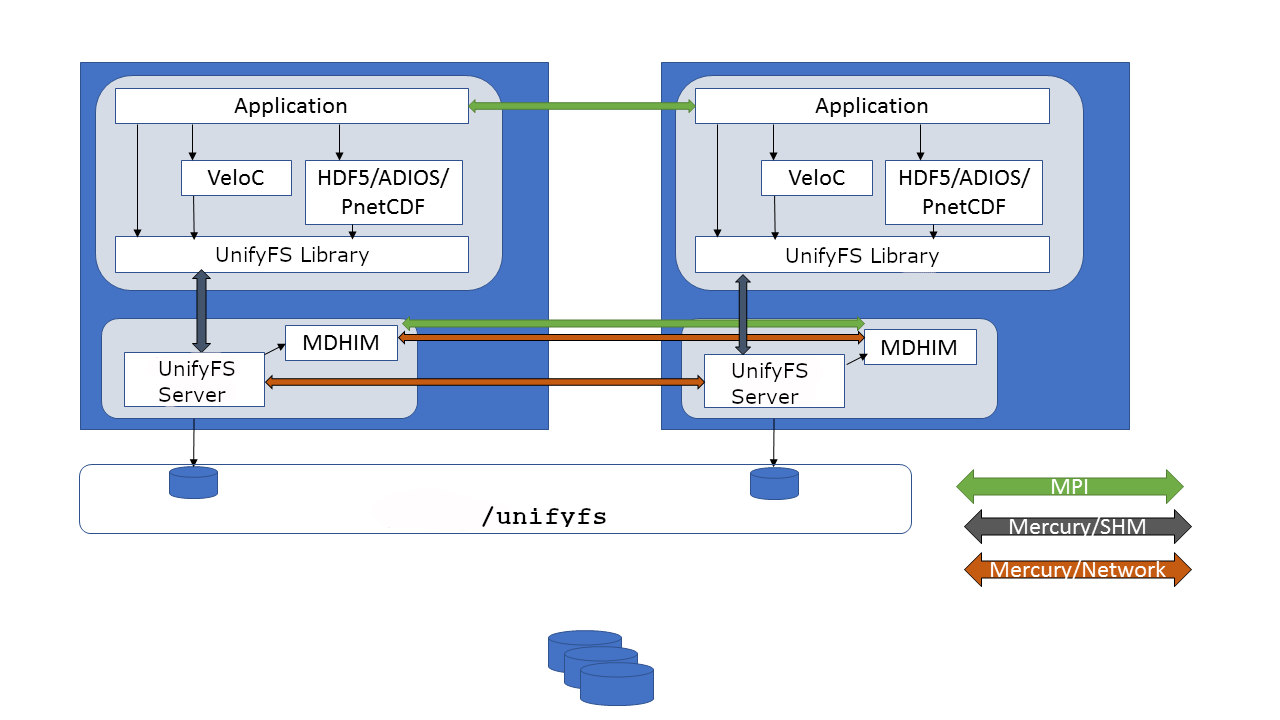
\includegraphics[width=4in]{projects/2.3.4-DataViz/2.3.4.15-HDF5-UnifyCR/milestone2}
        \caption{\label{fig:milestone2} \textbf{UnifyFS Design.} The UnifyFS
instance consists of a dynamic library and a UnifyFS daemon that runs
on each compute node in the job. The library intercepts I/O calls to
the UnifyFS mount point from applications, I/O libraries, or VeloC and communicates them to the UnifyFS daemon that handles the I/O operation.}
\end{figure}


Our source code for UnifyFS is available on 
GitHub at \url{https://github.com/LLNL/UnifyFS}. 
\paragraph{Next Steps}

For our next milestone effort, we are focused on delivering a design for 
the UnifyFS API for use by HDF5 and other I/O libraries. Additionally, we are continuing work on 
integrating and supporting ECP collaborator software including:
I/O libraries HDF5, MPI-IO, PnetCDF, and ADIOS; improving
support for ECP VeloC; and targeting integration with ECP applications such as
E3SM, GEOS, and Chombo.
We also plan to release UnifyFS 1.0 early in the 2020 calendar year.



